\documentclass[a4paper,12pt,titlepage,finall]{article}

\usepackage[T1,T2A]{fontenc}     % форматы шрифтов
\usepackage[utf8]{inputenc}      % кодировка символов, используемая в данном файле
\usepackage[english, russian]{babel}      % пакет русификации
\usepackage{tikz}                % для создания иллюстраций
\usepackage{pgfplots}            % для вывода графиков функций
\usepackage{geometry}		     % для настройки размера полей
\usepackage{indentfirst}         % для отступа в первом абзаце секции
\usepackage{amsmath,amsthm,amssymb}
\usepackage{mathtext}
\usepackage{graphicx}

\usepackage{caption}
\usepackage{subcaption}
\usepackage{hyperref}
\graphicspath{ {./img} }

%Настройка листингов для языка C
\usepackage{xcolor}
\usepackage{listings}
\lstset{extendedchars=\true}

\definecolor{mGreen}{rgb}{0,0.6,0}
\definecolor{mGray}{rgb}{0.5,0.5,0.5}
\definecolor{mPurple}{rgb}{0.58,0,0.82}
\definecolor{backgroundColour}{rgb}{0.95,0.95,0.95}

\lstdefinestyle{CStyle}{
    backgroundcolor=\color{backgroundColour},   
    keywordstyle=\color{mGreen},
    numberstyle=\tiny\color{mGray},
    breakatwhitespace=false,         
    breaklines=true,                 
    captionpos=b,                    
    keepspaces=true,                 
    numbers=none,                    
    numbersep=5pt,                  
    showspaces=false,                
    showstringspaces=false,
    showtabs=false,                  
    tabsize=2,
    language=C,
    basicstyle=\footnotesize\ttfamily ,
    extendedchars=\true ,
}

% выбираем размер листа А4, все поля ставим по 3см
\geometry{a4paper,left=30mm,top=30mm,bottom=30mm,right=30mm}

\setcounter{secnumdepth}{0}      % отключаем нумерацию секций
\setcounter{tocdepth}{2}

\usepgfplotslibrary{fillbetween} % для изображения областей на графиках

\begin{document}
\begin{titlepage}
    \begin{center}
	{\small \sc Московский государственный университет \\имени М.~В.~Ломоносова\\
	Факультет вычислительной математики и кибернетики\\}
	\hrulefill
	\vfill
	{\large \bf Компьютерный практикум по учебному курсу}\\
	~\\
	{\Large \bf <<Суперкомпьютеры и Параллельная
обработка данных>>}\\ 
	~\\
	~\\
	~\\
	{\bf Разработка параллельной версии программы для вычисления определенного интеграла с использованием метода трапеций}\\
	~\\
	{\large \bf ОТЧЕТ}\\
	{\bf о выполненном задании}\\
	{студента 327 учебной группы факультета ВМК МГУ}\\
	{Галустова Артемия Львовича}
    \end{center}
    
    \begin{center}
	\vfill
	{\small гор. Москва\\2021 год}
    \end{center}
\end{titlepage}

\tableofcontents
\newpage
\section{Постановка задачи}
Рассматривается определенный интеграл на отрезке $[a,b]$ функции одной переменной $f(x)$:
\begin{align*}
\int^b_a f(x) dx
\end{align*}

В ходе решения задачи требуется:
\begin{enumerate}
\item Реализовать алгоритм вычисление определенного интеграла методом трапеций.
\item Используя стандарт OpenMP адаптировать программу для параллельных вычислений.
\item Сравнить скорость вычислений при разном размере входных данных и разном количестве потоков.
\item Установить оптимальное количество потоков для каждого выбранного объема данных и объяснить полученные зависимости.
\end{enumerate}
\newpage
\section{Описание метода решения}
Сущность метода трапеций заключается в замене в каждой ячейки сетки подынтегральной функции на многочлен первой степени, т.е. линейную функцию, проходящую через значения функции в соседних узлах сетки. Тогда площадь под графиком аппроксимируется трапецией. Для отрезка между узлами $x_n$ и $x_{n+1}$ имеет место
\begin{align*}
\int^{x_{n+1}}_{x_n} f(x) dx = \frac{f(x_{n+1}) + f(x_{n})}{2}(x_{n+1} - x_n) + E(f)
\end{align*}
Для всего интервала формула имеет вид:
\begin{align*}
\int^b_a f(x) dx = \frac{f(a)}{2} (x_1 - a) + \sum_{i=1}^{n-1} \frac{f(x_i)}{2} (x_{i+1} - x_{i-1}) + \frac{f(b)}{2} (b - x_{n-1})
\end{align*}
В данной реализации используется равномерная сетка, потому возможно применить формулу Котеса:
\begin{align*}
\int^b_a f(x)\,dx = h \left( \frac{f_0 + f_n}{2} + \sum_{i=1}^{n-1} f_i \right)
\end{align*}

\section{Решаемая задача}
Для тестирования производительности необходимо предоставить программе достаточно сложную задачу. В данном случае в качестве интегрируемой функции была выбрана функция $f(x) = asin(x) + e^x + H(x)$. Три суммируемые функции были дополнительно разложены в ряды, чтобы исследовать ситуацию, когда функция без аналитического представления:
\begin{align*}
\arcsin x &= \sum^{\inf}_{n=0} \frac{(2n)!}{4^n (n!)^2 (2n+1)} x^{2n+1} \\
H(x) &= \sum^{\inf}_{n=0} \frac{2}{n \pi} \sin nx\\
e^x &=  \sum^{\inf}_{n=0} \frac{x^n}{n!}
\end{align*}
Использовалась равномерные сетки с разбиением на $1000, 10 000, 100 000$ и $1 000 000$ узлов. Это позволило получить время выполнения алгоритма в пределах от $0.006$ секунд до $2$ минут.

\section{Параллелизация и оптимизация алгоритма}
Основной оптимизацией для программы стало предвычисление коэффициентов ряда. Это управляется семейством опций $\_PREPARE\_COEFFICIENTS$. Также была добавлена опция для тестирования с распараллеливанием циклов внутри функций $\arcsin x, H(x), e^x$. Использовалась клауза omp parallel for. Управляется семейством опций $\_SERIES\_PARALLEL$. Также был распараллелен основной цикл интегрирования при помощи клаузы omp parallel.  Полный код программы доступен в разделе <<\nameref{source}>>, а также онлайн по адресу \url{https://github.com/NotLebedev/integralsOpenMP}.

\section{Методика тестирования}
Для получения репрезентативных и точных результатов был использован следующий подход для тестирования. Вначале программа выполняет три "прогревочных" раунда вычислений. Их время не учитывается в результате. Затем программа выполняет 5 раундов вычислений и усредняет время их выполнения измеренное при помощи $omp\_get\_wtime()$. Между раундами осуществляется сброс предвычисленных коэффициентов рядов. Данное поведение включается опцией $BENCHMARK$. Количество раундов задаётся опциями $WARMUP\_ROUNDS\_CNT$ и $ROUNDS\_CNT$.

\newpage
\section{Тестируемые конфигурации и результаты}
Первым произведённым тестом было сравнение эффективности программ производимых компиляторами IBM XL C/C++ (xlc++) и GNU Compiler Collection (g++). Эффективность программ сравнивалась на разбиении на $100 000$ узлов с предвычислением коэффициентов, но без распараллеливания внутренних циклов.
\begin{figure}[h]
\centering
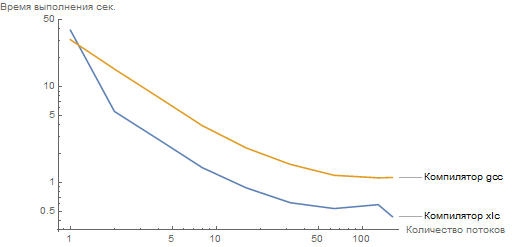
\includegraphics[width=0.7\textwidth]{plot_compilers.png}
\caption{Сравнение производительности программ собраных xlc и gcc}
\end{figure}
\par
Данное сравнение показывает существенное превосходство программ генерируемых xlc, потому все дальнейшие тесты были произведены с использование именно его.
\par
Для тестирования производительности были выполнены запуски по описанной выше методике с использованием трёх конфигураций:
\begin{itemize}
\item Без оптимизаций
\item С предвычислением коэффициентов
\item С предвычислением коэффициентов и параллелизацией внутренних циклов
\end{itemize}
\par
Были полученны следующие результаты:
\begin{table}[h]
\begin{tabular}{lllllll}
Optimizations & No        & Preopt     & Full       & No      & Preopt  & Full    \\
Series        & \multicolumn{3}{l}{1000}            & \multicolumn{3}{l}{10000}   \\
1             & 0.458736  & 0.114494   & 0.114606   & 9.12695 & 1.74852 & 7.8508  \\
2             & 0.229843  & 0.0554668  & 0.0575435  & 6.83397 & 1.65143 & 1.71756 \\
4             & 0.116875  & 0.0285275  & 0.0294921  & 5.7009  & 1.40852 & 1.47356 \\
8             & 0.0592613 & 0.0145033  & 0.0151491  & 5.18292 & 1.31402 & 1.33771 \\
16            & 0.0346732 & 0.00908069 & 0.00933806 & 5.15853 & 1.28186 & 1.31363 \\
32            & 0.0247849 & 0.00663345 & 0.179549   & 7.01354 & 1.99508 & 1.71551 \\
64            & 0.0209962 & 0.00600682 & 0.57386    & 11.5531 & 2.82944 & 1.91566 \\
128           & 0.0262914 & 0.00730744 & 0.572106   & 18.6607 & 5.68873 & 5.04403 \\
160           & 0.0423315 & 0.00730314 & 0.998173   & 31.6462 & 10.1763 & 10.1221
\end{tabular}
\end{table}
\begin{table}[h]
\begin{tabular}{lllllll}
Optimizations & No      & Preopt   & Full     & No      & Preopt  & Full    \\
Series        & \multicolumn{3}{l}{100000}    & \multicolumn{3}{l}{1000000} \\
1             & 128.656 & 38.9753  & 38.6009  &         & 110.277 & 114.706 \\
2             & 22.9074 & 5.53815  & 5.7552   &         & 55.3834 & 57.5783 \\
4             & 11.48   & 2.82549  & 2.94348  & 114.855 & 28.3578 & 29.4386 \\
8             & 5.80515 & 1.43243  & 1.48801  & 57.9605 & 14.3287 & 14.8846 \\
16            & 3.33129 & 0.880636 & 0.920509 & 33.3129 & 8.83835 & 9.09575 \\
32            & 2.29806 & 0.616865 & 0.647431 & 22.9805 & 6.18621 & 6.39415 \\
64            & 1.85798 & 0.535527 & 0.562976 & 18.5612 & 5.38622 & 5.62526 \\
128           & 1.95903 & 0.588818 & 0.624994 & 19.9604 & 6.03441 & 6.31218 \\
160           & 1.52373 & 0.441483 & 0.475114 & 15.4235 & 4.45109 & 4.81803
\end{tabular}
\end{table}
\newpage
\par
Для наглядности на графиках:
\begin{figure}[h]
\centering
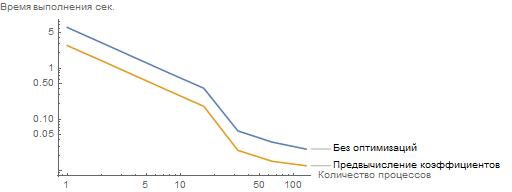
\includegraphics[width=0.7\textwidth]{plot1k.png}
\caption{Время выполнения для 1000 узлов}
\end{figure}
\begin{figure}[h]
\centering
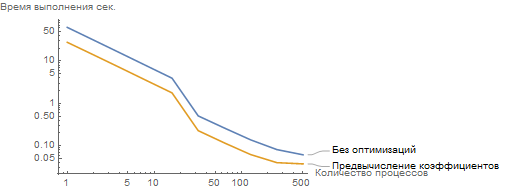
\includegraphics[width=0.7\textwidth]{plot10k.png}
\caption{Время выполнения для 10000 узлов}
\end{figure}
\begin{figure}[h]
\centering
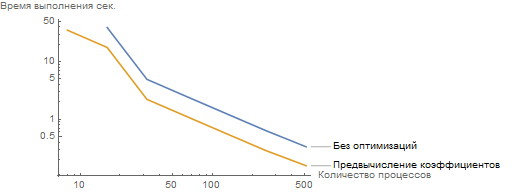
\includegraphics[width=0.7\textwidth]{plot100k.png}
\caption{Время выполнения для 100000 узлов}
\end{figure}
\begin{figure}[h]
\centering
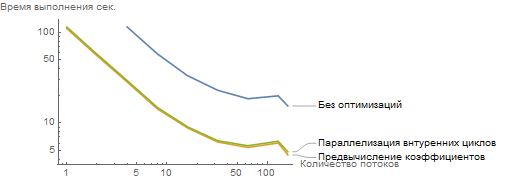
\includegraphics[width=0.7\textwidth]{plot1M.png}
\caption{Время выполнения для 1000000 узлов}
\end{figure}
\newpage
\section{Выводы}
Распараллеливание даёт существенный выигрыш при больших объемах вычислений. Это заметно как и в неэффективности использования значительного числа потоков для вычисления при малом числе узлов сетки, так и при применении параллелизации внутренних циклов. Предвычисление коэффициентов даёт существенное улучшение производительности чисто программными средствами. При малых объемах вычислений увеличение числа потоков приводит к ухудшению производительности после некоторого порога. Это связанно с тем, что накладные расходы на создание потоков и IPC начинают превышать выгоду от дальнейшего распараллеливания. Однако даже при значительных объемах вычислений производительность с некоторого момента перестаёт увеличиваться пропорционально увеличению кол-ва потоков. Это также связанно с накладными расходами, которые, не совсем превосходят преимущества параллелизации, но всё же частично уменьшают их. Также любопытно резкое замедление при использовании 128 потоков, время выполнения стабильно хуже чем у 64 и 160, что может объясняться особенностями архитектуры комплекса Polus. Полученные результаты демонстрируют, что для разных объемов вычислений целесообразны разные параметры параллелизации. Так для 1000 и 10000 узлов имеет смысл использовать 16-32 ядер, в то время как для 100000 и 1000000 узлов имеет смысл задействовать доступные ресурсы по максимуму. 
\newpage
\section{Полный листинг программы} \label{source}
\subsection{Файл main.cpp}
\lstinputlisting[style = CStyle]{../main.cpp}
\subsection{Файл functions/arcsin.cpp}
\lstinputlisting[style = CStyle]{../functions/arcsin.cpp}
\subsection{Файл $functions/heaviside\_step.cpp$}
\lstinputlisting[style = CStyle]{../functions/heaviside_step.cpp}
\subsection{Файл functions/exp.cpp}
\lstinputlisting[style = CStyle]{../functions/exp.cpp}
\end{document}